\documentclass{article}
\usepackage[utf8]{inputenc}
\usepackage{graphicx}
\usepackage{float}
\usepackage[x11names,table]{xcolor}
\usepackage{blindtext}
\usepackage[titletoc]{appendix}
\usepackage[nottoc]{tocbibind}
\usepackage{amsmath}
\usepackage{multirow}
\usepackage{lscape}
\usepackage{tikz}
\usepackage{subcaption}
\usetikzlibrary{automata, positioning, arrows, calc}
\usepackage{algorithm}
\usepackage{algpseudocode}
\usepackage{pifont}
\usepackage[TS1,T1]{fontenc}
\usepackage{array, booktabs}
\usepackage{caption}
\DeclareCaptionFont{blue}{\color{LightSteelBlue3}}


\numberwithin{table}{section}
\numberwithin{figure}{section}
\numberwithin{algorithm}{section}

\title{Self-organized task allocation for swarms in a Real Time Strategy game environment}
\author{Tomer Iwan}
\date{\today}

\begin{document}

\maketitle

\pagenumbering{roman}
% Abstract: generally, use the simple past 
% (or for a concise introductory phrase the present perfect); 
% for general statements and facts use the present tense.
\begin{abstract}

    
    Artificial Intelligence (AI) can be thought of as the study of machines that are capable of solving problems that require human level intelligence.
    It is a field in computer science which has seen a resurgence over the last few decades, both in academia and industry.
    Game AI (GAI) has long held the interest of researchers, with it being referred to as the tested for developing AI.
    Since the early 1950s, games have been a central theme of AI.
    Games address challenges that have great commercial, social, economic and scientific interest.
    Classical board games, such as chess, were long considered the drosophila of GAI, 
    due to their formal and highly constrained, yet complex, decision making nature.
    Over the years, researchers have achieving great results, achieving human level performances and beyond.
    As such, for decades research has been conducted on game playing.
    With the introduciton of video games, the efforts in GAI has increased rapidly.
    The complexity introduced by these games have been used to develop general AI.
    In video games with multiple agents, such as in Real Time Strategy (RTS) games, in combination with infinite game states, have added to the complexity.
    Novel AI solutions have been researched to address these challenging games.
    Swarm Intelligence (SI), a subcategory of AI, focuses on problem solving by means of collective behaviour of decentralized individual agents.
    Algorithms in SI, are inspired by the collective behavior of social organisms.
    The main principle of the collective behavior, is that it emerges from relatively simple actions between the indiviuals.
    \textcolor{blue}{---
    In this work, outlined is the general framework of interacting agents behaving as a swarm group in order to survive in a dangerous environment.
    The environment contains resources and threats, which are used to demonstrate classic swarm behaviours such as foraging.
    ---}
    Action selection of the agents are performed by means of Finite State Machines (FSM).
    The focus is put on the ability, of said swarm, to self-organize and distribute tasks among themselves.
    The obtained results show that the implementation has resulted in the expected behaviour to be emulated.
    This self-organized behaviour has lead to high level of fitness in the swarm population.
    
\end{abstract}

\newpage
\tableofcontents
\newpage
\listoffigures
\newpage

\listoftables
\newpage

\listofalgorithms
\addcontentsline{toc}{section}{List of Algorithms}
\newpage

\pagenumbering{arabic}
% Introduction: use a mixture of present and past tense; 
% the present tense is applied when you are talking about something that is always true; 
% the past tense is used for earlier research efforts, either by your own or by another group. 
% If the time of demonstration is unknown or not important, use the present perfect. 
% For the concluding statements of your introduction use the simple past; 
% you may use the past perfect, when you talk about something that was true in the past but is no longer so.
\section{Introduction} \label{section:introduction}
This thesis is framed within the general context of Artificial Intelligence (AI), 
focusing on the development of swarm intelligence (SI) in multi-agent games.
Early AI research concerned itself with the development of computational systems capable of displaying human-level intelligence.
The aim was to apply this intelligence in tasks of problem solving and decision making.
Such tasks were presented to the machines as a set of formal mathematical notations, 
which were able to be solved by means of symbol manipulation.
Due to this highly formalized framing of the problems, 
early AI was able to succeed in a large number of tasks.

Over the last couple of decades, the field has been thriving, 
with development happening at an increasing pace.
The efforts of AI research have not been limited to academia, 
as an increasing number of areas, unrelated to computer science, have adopted AI techniques, 
in the hope of increased performances.
The rapid advancements can be attributed to two main driving forces.
First and foremost, it is due to novel algoirthsm devides by the research community.
Secondly, the computational power of hardware, both in general and available to research, has increased, 
which allowed researchers to try increasingly more complex solutions.
These factors have allowed researchers to develop machines that have reached human-level intelligence and beyond in many fields, 
such as game-playing.

\textbf{Games}, in particular board games, have long been considered as the perfect research environment for AI methods.
This is partly due to them being a complex human activity.
However, the main reason is that they offer environments which are formal and highly constrained, 
suitable for decision making tasks. 

Game AI (GAI) is a sub-field of AI, which came to be quickly after AI itself.
It is a broad field, which is concerned with the challenge of developing AI for playing games at a high level, 
but also ventures into high level application, such as the automated generation of game aspects.

With the simultaneous rapid development of AI and the introduction of video games, 
the area of research has seen an overwhelming number of advancements in the last couple of years.
An early breakthrough occurred in the 1950s, when 
Shannon \cite{shannon1950xxii} 
developed a program for playing chess.
Other multi-player board games have been researched, for example, 
Othello \cite{buro2002improving}, 
Hex \cite{anshelevich2002hierarchical}, 
Shogi \cite{iida2002computer}, 
Go \cite{muller2002computer}, 
Backgammon \cite{tesauro2002programming}, 
Scrabble \cite{sheppard2002world} and 
Checkers \cite{chellapilla1999evolving}. 
Perhaps the most well-known feat in this field, 
was the victory of Deep Blue over world chess champion Garry Kasparov in 1997.
Another major achievement occurred in 2016 when DeepMind's AlphaGo defeated Lee Sedol in the game Go.

Numerous AI methods have been employed to tackle challenges in games, 
which include search algorithms, reinforcement- and deep learning, among others.
Many of these application, however, are concerned with the performance of a singular agent.

An emerging field, which explores the design of multi-agent systems, is swarm intelligence.
It is heavily inspired by the observation of collective behaviour of social insects, 
such as ants and bees.

Ants, for instance, are shown to use pheromone trails to communicate indirectly with each other, 
in tasks such as foraging food. 
Bees, on the other hand inform others in the swarm of new locations with an abundance of food, 
in a direct fashion through a specific dance.
The collective behaviour is not limited to foraging alone, 
as social insects are also known to build nests in cooperation.

Accordingly, other animal societies also display a form of collective behaviours, 
as can be seen in flocks of birds and schools of fish.

Although the individual members of the swarm are simple beings, 
together they are able to carry out complex tasks.
A key aspect of the collective behaviours, 
is that it emerges from relatively simple actions and interactions between individuals.

As such, these decentralized collective behaviours have caught the eye of AI researchers.
Thereforem, the design of applications in SI adhere to similar constraints.
As opposed to more traditional approaches, 
swarm intelligence does not make use of a sophisticated global controller to govern the behaviour of the system.
Instead, just as in nature, individual controllers, 
carrying out unsophisticated behaviours are employed, 
in order to achieve the desired behaviour by meand of cooperation.

\subsection{Research goals} \label{subsection:goals}
In recent years, the application of swarm intelligence in games has seen more research focus.
However, most research focuses on a limited number of traditional tasks that are to be performed by a swarm.
Having a more complex environment, 
with many actions available to the individual agents and the swarm has not seen much research as of yet.

This thesis will address the following research goals

\begin{enumerate}
    \item We aim to motivate work on swarm intelligence (SI) in video games
    \item We aim to apply SI to a novel developed multi-agent survival game
    \item We aim to focus on self-organized behaviour for task allocation
\end{enumerate}

\subsection{Thesis structure} \label{subsection:structure}

The thesis is organised as follows. 
In chapter \ref{section:background} background information is presented.
The chapter begins with a historic overview on Game AI, highlighting methods and major achievements.
Furthermore, we show the difference between academia and industry with regards to Game AI.
Additionally, the genre of Real Time Strategy (RTS) games is expanded upon.
The importance of projection in games is next touched upon.

Next, we define the basic concepts of swarm intelligence.
These include basic behaviours such as \textbf{foraging}, \textbf{flocking}, and \textbf{aggregation}.
This is followed by a description of self-organized behaviour, in particular task allocation.
The driving force behind actions in a swarm, Finite State Machines (FSM) is explained next.

Next in chapter \ref{section:methodology} the methods are presened. 
First, the game objectives are described. 
Next, the methods to build the game are described, which include the environment, camera and physics.
\textcolor{blue}{---
Further elements of the game are described in detail such as agents, enemies, and items.
---}
Finally, we describe the evaluation metric.

The results are presened in chapter \ref{section:results}, which are discussed in chapter \ref{section:discussion}.
The discussion will delve into the obtained results, coupling them to the research question which were defined in Section \ref{subsection:goals}.
Furthermore, we will look into the limitations of the proposed methods and will offer suggestions for future work.

Finally, the thesis is concluded in chapter \ref{section:conclusion}.

\section{Background} \label{section:background}
In this chapter we provide a theoretical basis on which to support the arguments and claims of the thesis. 
The chapter begins starts off with a brief overview of the history of Game AI, 
highlighting major achievements and the solutions applied.
Next, we shall define the basic concepts of swarm intelligence, 
and show how the field can be used in game-playing.


\subsection{Game AI} \label{subsection:game_ai}
See Table \ref{tab:timeline} for a recap of the timeline of game AI.

\newcommand{\foo}{\color{LightSteelBlue3}\makebox[0pt]{\textbullet}\hskip-0.5pt\vrule width 1pt\hspace{\labelsep}}

\begin{table}[H]
    \centering
    \renewcommand\arraystretch{1.4}\arrayrulecolor{LightSteelBlue3}
    \captionsetup{singlelinecheck=false, font=blue, labelfont=sc, labelsep=quad}
    \caption{Timeline of game AI}\vskip -1.5ex
    \begin{tabular}{@{\,}r <{\hskip 2pt} !{\foo} >{\raggedright\arraybackslash}p{5cm}}
    \toprule
    \addlinespace[1.5ex]
    1956 & The founding event of AI at The Dartmouth Summer Research Project on Artificial Intelligence\\
    1992 & \textbf{Backgammon}: TD-Gammon was developed, relying on ANN\\
    1994 & \textbf{Checkers}: Chinook defeats Marion Tinsley\\
    1996 & \textbf{Chess}: Garry Kasparov defeats IBM's Deep Blue (4 - 2)\\
    1997 & \textbf{Chess}: IBM's Deep Blue defeats Garry Kasparov (3.5 - 2.5)\\
    2014 & Google Deepmind uses raw pixel input to play Atari games\\
    2016 & \textbf{Go}: AlphaGo defeats Lee Sedol (4 - 1)\\
    2017 & \textbf{Go}: AlphaGo defeats Ke Jie (3 - 0)\\
    \end{tabular}
    \label{tab:timeline}
\end{table}

Game AI has a rich history, tracing back to the inception of the AI field itself.
Therefore, it can be considered an integral part of the field.
In the early days, research was focused on classic board games, such as backgammon, checkers and chess.
The reason being that these games, 
while being comprised of simple rules, 
presented a high level of complexity.
As such they have challenged the best human minds since their introduction.

In 1992, the backgammon software capable of playing at professional level, named TD-Gammon, was developed by Gerald Tesauro.
Playing against itself millions of time, the underlying artificial neural network was trained in order to achieve that level.

Two years later, Chinook, the checkers software managed to defeat the world checkers champion Marion Tinsley.
Chinook's achievement was based purely on domain knowledge by the creators, 
as the tree search used employed went through the pre-programmed actions.

Chess, in particular, long held the honour of being considered the "drosophila of AI", 
as it was considered to be a perfect testing ground for novel AI methods.

IBM developed the first software capable of displaying human-level chess playing, named \textit{Deep Blue}.
Deep Blue relied on a Minimax algorithm running on a supercomputer.
Furthermore, the software was given chess specific modifications.
IBM first attempted to defeat the chess grandmaster Garry Kasparov in 1996.
During this match, the world champion managed to defeat Deep Blue, winning four out of six rounds.
The rematch in the following year, saw IBM's Deep Blue emerge victorious, 
by winning twice, losing once and drawing three times in six rounds.
This historic event, is by many considered the day machines surpassed human intelligence.

Nowadays, the computing power of supercomputers is no longer necessary to play better than human players.
The software can be downloaded and run on vast majority of devices, such as laptops and smartphones.

With the game of chess being considered solved, 
the game of \textit{Go} was proposed to become the new benchmark for game-playing AI, 
due to its much larger search space compared to chess.
It was also considered to be the most challenging board game.

Two decades since the Deep Blue - Kasparov game, Google Deepmind's AlphaGo managed to defeat Lee Sedol in the game of Go.
The game, taking place in 2016, was won with a convincing score of 4 to 1.
The very next year, AlphaGo outclassed Ke Jie, then ranked number one in the world, by winning all three games.
The reason for its success, was the novel method of deep reinforcement learning.
In contrast to Deep Blue, Alpha Go was run on a single computer.

Now that the most complex board game was solved, there was no merit to create and solve a new board game.
A more complex game, would not be interesting for human players, and any achievement by a computer on such games would hold little significance.
Luckily for the field of game AI, there is more to games than the classical turn-based board games.

With the booming gaming industry bringing out large numbers of video games, 
there are endless new possibilities to develop AI to be able to play them.

Video games, as opposed to the board games, require a different kind of intelligence.
Instead of turn based decision making, the software needs to be able to decide in real time.
As such they pose as interesting testing field for AI. 
John McCarthy, one of the founding fathers of AI, \cite{mccarthy1998partial} even singled out the \textit{Lemmings} game as an important game in the field of Game AI, 
as early as 1998.
A couple of years later, Kendall et al. \cite{kendall2004scripting} used the game to demonstrate its relevance to Game AI.

In 2014, Google Deepmind developed a number of algorithms, which were able to use raw pixel input to play Atari games.
\textcolor{blue}{---To be continued ---}

% add some more.
% to methodology.
Check out this book by Buckland \cite{buckland2005programming}.
% 

\subsection{Gap between academia and industry} \label{subsection:gap}
Yannakakis and Togelius \cite{yannakakis2018artificial} have shown that the development of Game AI is often not implemented in the gaming industry.

A prominent reason is that, in the gaming industry, it is not considered desired to have an AI that is perfect in playing.
Having a perfect playing NPC, would make the game too hard and thus less enjoyable to the player.

There needs to be a happy medium, where AI is deployed that is challenging, but systematically makes sub-optimal decisions.

% cunha2015swarm
\textcolor{red}{---
The AI techniques in commercial games are often simplistic in comparison to the ones developed and used in academic research or in other industrial applications. 
This fact should not be understood as AI in games is poorly done, 
as we could tell from the previous given examples. 
Even back in the 2000s, when there was a big funneling of effort and resources to graphical fidelity, 
there was a set of well established techniques widely used by game developers — e.g. 
Fuzzy State Machines, 
the A* Path-Finding
algorithm, 
and the BOIDS flocking of Craig Reynolds are examples of such techniques.
On a side note, we find it relevant to point out that these techniques were (and still are) so useful in the industry that there were some who thought of creating 
Software Development Kits(SDKs) with generic implementations of AI components, with the intention of lowering the game’s development times[32].
Not many people ended up using these SDKs, because of their lack of flexibility — they were not usable without a great deal of effort from the developer, 
often requiring specific solutions for each problem to solve. 
Ultimately these SDKs did not solve any problem.
Despite these early issues, nowadays, the average household computer has much higher specifications. This, aligned with the development and improvement of the Graphics Processing Unit(GPU),
made it possible to allocate a processing unit dedicated to graphics, freeing (some) of the other cores for general processing. 
All these advancements make it possible to further develop and to use higher demanding AI techniques inside our games, without breaking the performance nor the experience. 
Also, the current graphical level is so high that a game is expected to have some awesome or innovative gameplay mechanic, and/or noticeable good AI.
---}


\subsection{Swarm Intelligence} \label{subsection:swarm_intelligence}
Before blindtext I will cite this paper by Eliseo \cite{brambilla2013swarm}.
% cunha2015swarm
\textcolor{red}{---
It is a well known fact that Man learned a lot from studying natural systems. 
This is also true for Computer Science[38], as the studies derived from natural system inspired the development of such algorithm models like 
artificial neural networks, 
evolutionary computation, 
swarm intelligence, artificial immune systems, 
and fuzzy state machines. 
These mentioned breakthroughs in computer science are the respective models of biological neural networks, 
evolution, 
swarm behavior of social organisms, 
natural immune systems, 
and human thinking processes.
---}

\textcolor{red}{---
From the studies on social organisms, it became evident that their ability to perform complex tasks had the interactions between the individuals of the swarm in its core. 
This means, that the complexity was not innate within any of the individuals, 
but rather present when analyzing their behavior as a whole.
The interaction in these biological swarm systems may be direct — through the natural senses of touch,
smell, hear or seeing — or indirect — through changes in the environment. 
The ability to perform complex tasks as a result of individual independent labor is called emergence and it is not easy to predict or deduct the complex resulting behavior from observing the simple behavior of the individuals. 
Engelbrecht et al.[38] define emergence as the process deriving some new and coherent structures, patterns and properties (or behaviors) in a complex system — 
structures, patterns and properties (or behaviors)
that come to be without the presence of a central commanding unit delegating or tasks to the individuals.
---}


\textcolor{red}{---
Swarm Intelligence (SI) is the terminology used to describe the problem-solving behavior emergent from the interaction between agents within a swarm (or colony). 
In the same way that Computer Swarm Intelligence is the terminology used to the algorithmic representations that model those same emergent behavior.
SI studies ways to implement collective behavior resulting from decentralized and self-organized systems. 
Even though small and with limited sensory and cognitive skills, 
these insects are able to form colonies and work together in order to persevere. 
This perseverance often implies the need to perform complex tasks as a group, 
such as food foraging, brood clustering, and construction and maintenance of the nest. 
The reason why this is so impressive, 
is because these insects are able to perform all these tasks without a central unit controlling or defining the objectives, 
nor assigning each member of the colony to a specific task.
---}

\textcolor{red}{---
We can exemplify this concept with ants, for example. 
Like other insects, ants have several built-in systems that allow them to be so productive[25], and have helped with problem. 
By defining a clear objective, 
like foraging for food or building a nest, 
they help the colony units understand their purpose.
They are committed in the greater good, 
even if they may seem to wander aimlessly on their own, 
they are continuously searching for ways to serve the colony. 
Ants live in an empowering culture, 
which means that each ant (or each colony unit) is allowed to try and experiment as many possibilities as possible to reach a goal, 
without adverse consequences for failure — this empowerment may result in finding a better supply of food, for example. 
And, finally, ants dispose of an automatic communication system that they simply cannot turn off — 
this allows any ant who follows is always benefited by the information gathered by previous ants. 
This allows them to efficiently search for an optimal or near-optimal solution for their goal.
---}

% brambilla2013swarm
See Sahin's \cite{csahin2004swarm} description of swarm robotics.
\textcolor{red}{---
The main characteristics of a swarm robotics system are the following:
\begin{itemize}
    \item robots are autonomous;
    \item robots are situated in the environment and can act to modify it;
    \item robots’ sensing and communication capabilities are local;
    \item robots do not have access to centralized control and/or to global knowledge;
    \item robots cooperate to tackle a given task.
\end{itemize}
---}
% csahin2004swarm see source for full description

\textcolor{red}{---
The main inspiration for swarm robotics comes from the observation of social animals. 
Ants, bees, birds and fish are some examples of how simple individuals can become successful when they gather in groups. 
The interest towards social animals stems from the fact that they exhibit a sort of swarm intelligence (Bonabeau et al., 1999; Dorigo and Birattari, 2007). 
In particular, the behavior of groups of social animals appear to be robust, scalable and flexible.
Robustness is the ability to cope with the loss of individuals. 
In social animals, robustness is promoted by redundancy and the absence of a leader. 
Scalability is the ability to perform well with different group sizes. 
The introduction or removal of individuals does not result in a drastic change of the performance of a swarm. 
In social animals, scalability is promoted by local sensing and communication. 
Flexibility is the ability to cope with a broad spectrum of different environments and tasks. 
In social animals, flexibility is promoted by redundancy, simplicity of the behaviors and mechanisms such as task allocation. 
A detailed analysis of robustness, scalability and flexibility in social animals has been carried out by Camazine et al. (2001).
By taking inspiration from social animals, 
swarm robotics aims at developing robotics systems that exhibit swarm intelligence features similar to those that characterize social animals. 
In particular, swarm robotics systems are meant to be robust, scalable and flexible.
---}

\textcolor{red}{---
yet their system-level functioning is robust, flexible and scalable. 
Such properties are acknowledged to be desirable for also multi-robot systems, 
and can be stated as motivations for the swarm robotics approach:
---}

See the book from Eberhart et al. on swarm intelligence \cite{eberhart2001swarm}.


% uncited: bollam2016swarm
% section 3.4
\textcolor{red}{---
While implementing artificial swarms we need to consider several things like the issues which may arise during agent’s behavior within the swarm. 
There are few base conditions which need to be maintained to achieve the correct swarming behaviors.
There is artificial swarm program developed by Craig Reynolds \cite{reynolds1987flocks} in order to simulate the birds flocking behavior, called Boids. 
This is abbreviation for “bird-oid object” which means bird like objects.
This model is constructed based on a set of simple rules and this can be extended to complex set
of rules. 
Simple rules applied to the Boids
\begin{itemize}
    \item separation: direct to avoid crowding local flock mates
    \item alignment: direct towards the average heading of local flock mates
    \item cohesion: direct to move toward the average position of local flock mates
\end{itemize}
We can add few additional complex conditions to make it more reliable like obstacle avoidance and task completion.
---}
% bollam2016swarm p.12/62
\textcolor{red}{---
Swarm can therefore be viewed as a cluster of agents.
Viewing swarms as such, makes it possible to see that swarm are able to break off into smaller clusters.
This may occur if the swarm is too large, or when numerous agents are needed simultaniously to perform an action.
See Equation \ref{equations:cluster_swarm} and Figure \ref{fig:cluster_swarm}.
---}
\begin{equation}
    Swarm^{\mu}(new) \cup Swarm^{v} = Swarm^{\mu}(new)
    \label{equations:cluster_swarm}
\end{equation}


\begin{equation}
    Swarm^{\mu}(new) \cup Swarm^{v} = Swarm^{\mu}(new)
    \label{equations:cluster_swarm}
\end{equation}



% blum P. 46 on ACO
\textcolor{red}{---
Ant colony optimization (ACO) [52] was one of the first techniques for approximate optimization inspired by swarm intelligence. 
More specifically, ACO is inspired by the foraging behavior of ant colonies. 
At the core of this behavior is the indirect communication between the ants by means of chemical pheromone trails, 
which enables them to find short paths between their nest and food sources. 
---}

\subsection{Foraging} \label{subsection:foraging}
% hamann2018swarm
\textcolor{red}{---
Foraging behaviors are omnipresent in the animal world because all animals need nutrition. 
We are interested in foraging strategies of social insects.
We skip a sophisticated review of the biological literature here. 
From the modeling perspective of swarm robotics, for example, 
the foraging model of Schmickl and Crailsheim [343] for honeybees is interesting and so is also the relevance of noise in the decision-making process of foraging ants as reported by Meyer et al. [274]. 
The work by Jackson et al. [194] was mentioned above in Sect. 4.3.1 and it is relevant here because it explains how foraging ants navigate their trail network.
Foraging is also of interest in robotics even though our robots do usually not eat. 
Instead you should interpret foraging as a search and retrieval behavior. 
There are of course many tasks, such as search and rescue, that are related to foraging and of interest in robotics. 
All these tasks can be done by a single robot or a robot swarm.
Interesting for modeling in swarm robotics is the model by Lerman and Galstyan [236]. 
They investigate the effect of interference in a foraging group of robots. 
Robots search objects, pick them up, and bring them to a certain target area. 
It is expected that there can be quite some traffic at that target area, which may trigger interference between robots. 
For example, they find the typical swarm performance curves as described in Chap. 1. Hamann and Wörn [175] report a spatial model of a foraging behavior based on pheromones.
Probably one of the earliest works on foraging in robots was reported by Sugawara and Sno [369] and Sugawara et al. [368]. 
They report successful experiments with five robots and find that cooperation is effective.
Mayet et al. [259] report a method to emulate pheromones for a foraging behavior similar to ants based on ultraviolet light and glow paint (see Fig. 4.10). 
They use extended e-puck robots. Robots can “draw” trails on the ground by lighting their ultraviolet LED. 
The trail is then detected by vision. 
The approach also includes a light beacon to emulate a compass.
The above mentioned approach by Nouyan et al. [295] is one of the most sophisticated experiments in swarm robotics. 
The robots form chains, search for an object, once the object is found they collectively transport it along the chain of robots back to their base station.
The probably most complex foraging behavior reported in swarm robotics is that of Dorigo et al. [98]. 
It was done within the Swarmanoid project that investigated heterogeneous swarm robots. 
The eye-bot (quadrotor), hand-bot (robot with grippers), and foot-bot (similar to the s-bot) cooperate to pick up a book from a shelve. 
First they have to find it, which is done by the eye-bot, 
then they form a relay-station line of foot-bots, 
collectively transport a hand-bot to the shelf, 
and the hand-bot finally picks up the book.
---}


\subsection{Flocking} \label{subsection:flocking}
% https://en.wikipedia.org/wiki/Flocking_(behavior)
\textcolor{red}{---
Flocking is the behavior exhibited when a group of birds, called a flock, are foraging or in flight.
From the perspective of the mathematical modeller, "flocking" is the collective motion by a group of self-propelled entities, 
and is a collective animal behavior exhibited by many living beings such as birds, fish, bacteria, and insects.
It is considered an emergent behavior arising from simple rules that are followed by individuals and does not involve any central coordination.
---}

\textcolor{red}{---
Basic models of flocking behavior are controlled by three simple rules:
\begin{enumerate}
    \item Separation – avoid crowding neighbours (short range repulsion)
    \item Alignment – steer towards average heading of neighbours
    \item Cohesion – steer towards average position of neighbours (long range attraction)
\end{enumerate}
With these three simple rules, the flock moves in an extremely realistic way, 
creating complex motion and interaction that would be extremely hard to create otherwise.
---}

\textcolor{blue}{---
See the paper by Reynolds on boids \cite{reynolds1987flocks}.
Not sure if exactly in flocking but look at the ant study by Goss et al. \cite{goss1989self}.
---}

% https://en.wikipedia.org/wiki/Swarm_behaviour
\textcolor{red}{---
The mathematical model presented in this paper is as follows.
Each bird-oid object (boid) has to adhere to three rules, which are:
\begin{itemize}
    \item Move in the same direction as their neighbours
    \item Remain close to their neighbours
    \item Avoid collisions with their neighbours
\end{itemize}
---}

\subsection{Aggregation} \label{subsection:aggregation}

\textcolor{blue}{---
Another book to look into is by Hamann et al. \cite{hamann2018swarm}.
Yet another book by Blum et al. \cite{blum2008swarm}.
---}

% brambilla
Aggregation is a widespread collective behaviour in nature.
Other than in various insect species, the behaviour can also be observed in birds, fish and bacteria \cite{camazine2020self}.
The goal of aggregation is to group all members of a swarm in a region of the environment.
While simple, the behaviour is extremely useful, as it allows individuals, within a swarm, to get sufficiently close in order to interact.

\subsection{Task allocation} \label{subsection:task_allocation}
% yang2009swarm

\textcolor{red}{---
In swarm robotic system, task allocation can also be treated as labor division or role assignment. 
Usually, individual robot has equal capability for the tasks to be executed.
A simple and decentralized task allocation mechanism based on individual activation-thresholds which is originated from \cite{bonabeau1998fixed}. 
Each robot is assigned with a threshold value  and the robot will decide to go collect food-items if the energy level of the nest is less than the threshold.
---}

\textcolor{red}{---
The challenge of properly partitioning and allocating work in a swarm is important, difficult, 
and is an aspect of swarm robotics that comes with a lot of algorithmic features. 
Division of labor means the work is organized, 
not everyone is doing the same tasks, and consequently the work needs to be usefully distributed among the workers. 
Task partitioning is the problem of defining smaller pieces of work (tasks). 
They should of course be self-contained and each task should have similar requirements and a similar volume. 
Task allocation is then the problem of assigning tasks to the robots, hopefully in an efficient way. 
Both task partitioning and task allocation can be done offline (before deploying the system) and online (at runtime). 
An offline approach is simpler but an online approach allows for adaptations to dynamic changes. 
If the task allocation is dynamic, then a strategy for task switching is required. 
One wants to avoid frequent switching because each switch may come with a certain overhead.
---}

Bonabeau et al. \cite[Chapter~3]{bonabeau1999swarm} goes into detail how insect colonies divide tasks.
See also from the same author \cite{bonabeau1998fixed}.

Garattoni et al. \cite{garattoni2018autonomous} demonstrated how autonomous task sequencing could be applied in a robot swarm.

Ducatelle et al. did the following \cite{ducatelle2009new}.

Yang et al. demonstrated that a simple threshold model could be effective in task allocation \cite{yang2009swarm}.

% brambilla
\textcolor{red}{---
Task allocation is a collective behavior in which robots distribute themselves over different tasks. 
The goal is to maximize the performance of the system by letting the robots dynamically choose which task to perform.
---}

\textcolor{red}{---
Task allocation can be observed in natural systems such as ant and bee colonies – e.g., Theraulaz et al. (1998). 
For example, in ant or bee colonies, part of the swarm can perform foraging while another part looks after the larvae. 
Task allocation is not fixed but can change over time.
---}

\textcolor{red}{---
In swarm robotics, task allocation is mainly obtained through the use of probabilistic finite state machines. 
To promote specialization, 
the probabilities of selecting one of the available tasks are either different among the robots or they can change in response to task execution or messages from other robots. 
In swarm robotics, task allocation has been studied mainly on robots performing foraging.
---}

\subsection{Finite State Machines} \label{subsection:FSM}
% buckland
\textcolor{red}{---
Historically, a finite state machine is a rigidly formalized device used by mathematicians to solve problems. 
The most famous finite state machine is probably Alan Turing’s hypothetical device: 
the Turing machine, 
which he wrote about in his 1936 paper, 
“On Computable Numbers.” 
This was a machine presaging modern-day programmable computers that could perform any logical operation by reading, writing, 
and erasing symbols on an infinitely long strip of tape. 
Fortunately, as AI programmers, we can forgo the formal mathematical definition of a finite state machine; 
a descriptive one will suffice:
A finite state machine is a device, or a model of a device, 
which has a finite number of states it can be in at any given time, 
and can operate on input to either make transitions from one state to another or to cause an output or action to take place. 
A finite state machine can only be in one state at any moment in time.
---}

See Figure \ref{fig:simple_FSM} for a simple example of a FSM for a light bulb. 
When the light bulb is in the on state, the action to turn it off triggers the off state.
Conversely, turning the light bulb on in the off state, changes the state to on.

\begin{figure}[H]
    \centering
    

\tikzset{every picture/.style={line width=0.75pt}} %set default line width to 0.75pt        

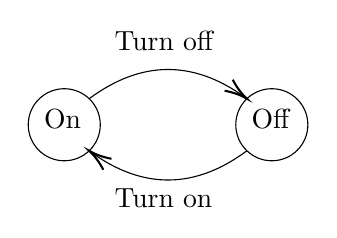
\begin{tikzpicture}[x=0.75pt,y=0.75pt,yscale=-1,xscale=1]
%uncomment if require: \path (0,199); %set diagram left start at 0, and has height of 199


% Text Node
\draw    (133, 145.5) circle [x radius= 17.36, y radius= 17.36]   ;
\draw (122,137) node [anchor=north west][inner sep=0.75pt]   [align=left] {On};
% Text Node
\draw    (233, 145.5) circle [x radius= 17.36, y radius= 17.36]   ;
\draw (222,137) node [anchor=north west][inner sep=0.75pt]   [align=left] {Off};
% Text Node
\draw (156,99) node [anchor=north west][inner sep=0.75pt]   [align=left] {Turn off};
% Text Node
\draw (156,175) node [anchor=north west][inner sep=0.75pt]   [align=left] {Turn on};
% Connection
\draw    (145,132.96) .. controls (169.82,114.56) and (194.66,114.19) .. (219.48,131.85) ;
\draw [shift={(221,132.96)}, rotate = 216.55] [color={rgb, 255:red, 0; green, 0; blue, 0 }  ][line width=0.75]    (10.93,-3.29) .. controls (6.95,-1.4) and (3.31,-0.3) .. (0,0) .. controls (3.31,0.3) and (6.95,1.4) .. (10.93,3.29)   ;
% Connection
\draw    (221,158.04) .. controls (196.18,176.44) and (171.34,176.81) .. (146.52,159.15) ;
\draw [shift={(145,158.04)}, rotate = 396.55] [color={rgb, 255:red, 0; green, 0; blue, 0 }  ][line width=0.75]    (10.93,-3.29) .. controls (6.95,-1.4) and (3.31,-0.3) .. (0,0) .. controls (3.31,0.3) and (6.95,1.4) .. (10.93,3.29)   ;

\end{tikzpicture}

    \caption{Light bulb FSM}
    \label{fig:simple_FSM}
\end{figure}




% yannakis
\textcolor{red}{---
FSMs belong to the expert-knowledge systems area and are represented as graphs. 
An FSM graph is an abstract representation of an interconnected set of objects, symbols, events, actions or properties of the phenomenon that needs to be ad- hoc designed (represented). 
In particular, the graph contains nodes (states) which embed some mathematical abstraction and edges (transitions) which represent a conditional relationship between the nodes. 
The FSM can only be in one state at a time; the current state can change to another if the condition in the corresponding transition is fulfilled. 
In a nutshell, an FSM is defined by three main components:
---}

\textcolor{red}{---
\begin{itemize}
    \item A number of states which store information about a task—e.g., you are currently on the explore state.
    \item A number of transitions between states which indicate a state change and are described by a condition that needs to be fulfilled—e.g., if you hear a fire shot, move to the alerted state.
    \item A set of actions that need to be followed within each state—e.g., while in the explore state move randomly and seek opponents.
\end{itemize}
---}

% 532 = Michele Pirovano. The use of Fuzzy Logic for Artificial Intelligence in Games. Technical report, University of Milano, Milano, 2012.
% 109 = AlexJ.Champandard.AIgamedevelopment:Syntheticcreatureswithlearningandreactive behaviors. New Riders, 2003.
\textcolor{red}{---
FSMs are incredibly simple to design, implement, visualize, and debug. Further they have proven they work well with games over the years of their co-existence. 
However, they can be extremely complex to design on a large scale and are, thereby, computationally limited to certain tasks within game AI. 
An additional critical limitation of FSMs (and all ad-hoc authoring methods) is that they are not flexible and dynamic (unless purposely designed). 
After their design is completed, tested and debugged there is limited room for adaptivity and evolution. 
As a result, FSMs end up depicting very predictable behaviors in games. 
We can, in part, overcome such a drawback by representing transitions as fuzzy rules [532] or probabilities [109].
---}

\subsection{Projection} \label{subsection: projection}
In general, there are three types of projection in games to be distinguished, which are orthographic, oblique and perspective projections \cite{salomon2007transformations}.

In orthographic, we can distinguish three methods, which are isometric, dimetric and trimetric.


% use salomon source to show matrix manipulation for the projections.
Assume the vector $(1, 0, 0)$
% see Table \ref{tab:projections-table}.
% insert table pros, cons

% \begin{landscape}
    \newcommand{\ra}[1]{\renewcommand{\arraystretch}{#1}}
    \begin{table*}\centering
        \caption{An overview of the properties of the different projections}
        \label{tab:projections-table}
        \ra{1.3}
            \begin{tabular}{@{}rrrrcrrrcrrr@{}}\toprule
            & \multicolumn{3}{c}{$w = 8$} & \phantom{abc}& \multicolumn{3}{c}{$w = 16$} &
            \phantom{abc} & \multicolumn{3}{c}{$w = 32$}\\ \cmidrule{2-4} \cmidrule{6-8} \cmidrule{10-12}
            & $t=0$ & $t=1$ & $t=2$ && $t=0$ & $t=1$ & $t=2$ && $t=0$ & $t=1$ & $t=2$\\ \midrule
            $dir=1$\\
            $c$ & 0.0790 & 0.1692 & 0.2945 && 0.3670 & 0.7187 & 3.1815 && -1.0032 & -1.7104 & -21.7969\\
            $c$ & -0.8651& 50.0476& 5.9384&& -9.0714& 297.0923& 46.2143&& 4.3590& 34.5809& 76.9167\\
            $c$ & 124.2756& -50.9612& -14.2721&& 128.2265& -630.5455& -381.0930&& -121.0518& -137.1210& -220.2500\\ $dir=0$\\
            $c$ & 0.0357& 1.2473& 0.2119&& 0.3593& -0.2755& 2.1764&& -1.2998& -3.8202& -1.2784\\
            $c$ & -17.9048& -37.1111& 8.8591&& -30.7381& -9.5952& -3.0000&& -11.1631& -5.7108& -15.6728\\
            $c$ & 105.5518& 232.1160& -94.7351&& 100.2497& 141.2778& -259.7326&& 52.5745& 10.1098& -140.2130\\ \bottomrule
            \end{tabular}
    \end{table*}
\end{landscape}

\tikzset{-, every picture/.style={line width=0.75pt}} %set default line width to 0.75pt        
\begin{figure}[H]
    \centering
    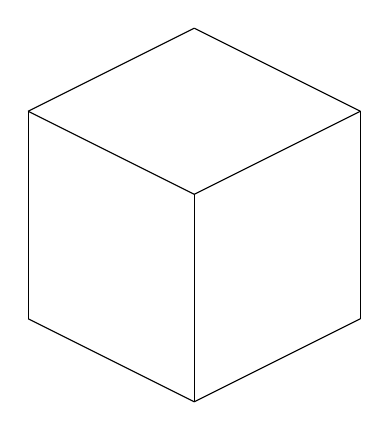
\begin{tikzpicture}[x=0.75pt,y=0.75pt,yscale=-1,xscale=1]
        %uncomment if require: \path (0,300); %set diagram left start at 0, and has height of 300

        %Straight Lines [id:da052099186519106055] 
        \draw    (234,86) -- (234,186) ;
        %Straight Lines [id:da6296181006552015] 
        \draw    (234,86) -- (314,126) ;
        %Straight Lines [id:da34479128766647027] 
        \draw    (314,126) -- (394,86) ;
        %Straight Lines [id:da7728351637240529] 
        \draw    (314,46) -- (234,86) ;
        %Straight Lines [id:da3095482376565484] 
        \draw    (314,46) -- (394,86) ;
        %Straight Lines [id:da019510812171401604] 
        \draw    (234,186) -- (314,226) ;
        %Straight Lines [id:da7918604023131788] 
        \draw    (394,186) -- (314,226) ;
        %Straight Lines [id:da43921670234898924] 
        \draw    (394,86) -- (394,186) ;
        %Straight Lines [id:da07253833503340212] 
        \draw    (314,126) -- (314,226) ;

    \end{tikzpicture}
    \caption{Isometric projection}
    \label{fig:isometric}
\end{figure}

\tikzset{-, every picture/.style={line width=0.75pt}} %set default line width to 0.75pt        
\begin{figure}[H]
    \centering
    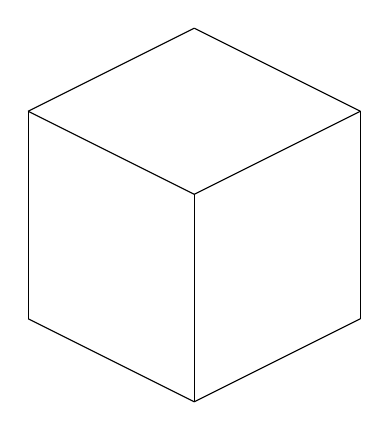
\begin{tikzpicture}[x=0.75pt,y=0.75pt,yscale=-1,xscale=1]
        %uncomment if require: \path (0,300); %set diagram left start at 0, and has height of 300

        %Straight Lines [id:da052099186519106055] 
        \draw    (234,86) -- (234,186) ;
        %Straight Lines [id:da6296181006552015] 
        \draw    (234,86) -- (314,126) ;
        %Straight Lines [id:da34479128766647027] 
        \draw    (314,126) -- (394,86) ;
        %Straight Lines [id:da7728351637240529] 
        \draw    (314,46) -- (234,86) ;
        %Straight Lines [id:da3095482376565484] 
        \draw    (314,46) -- (394,86) ;
        %Straight Lines [id:da019510812171401604] 
        \draw    (234,186) -- (314,226) ;
        %Straight Lines [id:da7918604023131788] 
        \draw    (394,186) -- (314,226) ;
        %Straight Lines [id:da43921670234898924] 
        \draw    (394,86) -- (394,186) ;
        %Straight Lines [id:da07253833503340212] 
        \draw    (314,126) -- (314,226) ;

    \end{tikzpicture}
    \caption{Dimetric projection}
    \label{fig:dimetric}
\end{figure}
% make dimetric
\tikzset{-, every picture/.style={line width=0.75pt}} %set default line width to 0.75pt        
\begin{figure}[H]
    \centering
    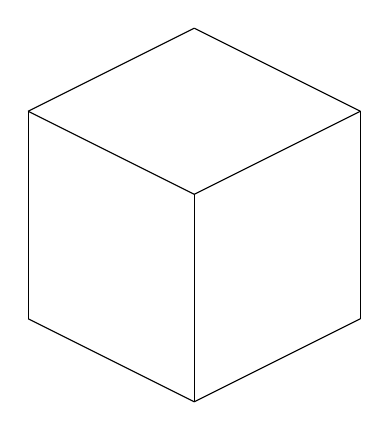
\begin{tikzpicture}[x=0.75pt,y=0.75pt,yscale=-1,xscale=1]
        %uncomment if require: \path (0,300); %set diagram left start at 0, and has height of 300

        %Straight Lines [id:da052099186519106055] 
        \draw    (234,86) -- (234,186) ;
        %Straight Lines [id:da6296181006552015] 
        \draw    (234,86) -- (314,126) ;
        %Straight Lines [id:da34479128766647027] 
        \draw    (314,126) -- (394,86) ;
        %Straight Lines [id:da7728351637240529] 
        \draw    (314,46) -- (234,86) ;
        %Straight Lines [id:da3095482376565484] 
        \draw    (314,46) -- (394,86) ;
        %Straight Lines [id:da019510812171401604] 
        \draw    (234,186) -- (314,226) ;
        %Straight Lines [id:da7918604023131788] 
        \draw    (394,186) -- (314,226) ;
        %Straight Lines [id:da43921670234898924] 
        \draw    (394,86) -- (394,186) ;
        %Straight Lines [id:da07253833503340212] 
        \draw    (314,126) -- (314,226) ;

    \end{tikzpicture}
    \caption{Trimetric projection}
    \label{fig:trimetric}
\end{figure}
% make trimetric


In \textit{isometric} projections all sides seem to have the same length. 
% text above from salomon source


Have a look at the three orthographic projections in Figure \ref{fig:isometric}, Figure \ref{fig:dimetric} and Figure \ref{fig:trimetric}.

% for isometric show zig-zag vs diamond approach
% In isometric maps, we can furthermore distinguish staggered and diamond representations.
% Diamond maps are typically used in RTS and Tactical Combat types games 
% whereas Staggered/Block maps tend to be used for RPG's and Turn-Based Strategy games.
Here is another source for axonometry and in particular isometry \cite{krikke2000axonometry}.

% from krikke2000axonometry, try to emulate in tikz
\begin{figure}[H]
    \centering
    
    \includegraphics{graphics/screenshots/world.png}
    \caption{Isometric world}
    \label{fig:isometric_world}
\end{figure}

% from krikke plagianus
% recreate with tikz

% https://isometric-tiles.readthedocs.io/en/latest/
\textcolor{red}{---
\textbf{Isometric coordinates}.
Traditional top-down or side-view games normally work in a traditional grid. Graphics are placed in these grid locations. 
Each graphic is a rectangle, and sometimes they are referred to as “tiles.”
Converting between grid locations and the screen’s pixel coordinates are reasonably straight-forward.
Another type of 2D game uses “Isometric Tiles.” 
Here, we can fake a 3D view with 2D graphics. We do that by tilting the grid 45 degrees. 
Each tile then becomes a diamond.
---}

\textcolor{red}{---
In order to transform the tiles to pixels on the screen the following variables need to be defined:
\begin{itemize}
    \item tilewidth = width of each tile in pixels
    \item tileheight = height of each tile in pixels
    \item tilex = x-coordinate of the tile, in tiles
    \item tiley = y-coordinate of the tile, in tiles
    \item width = width of the map, in tiles
    \item height = hieght of the map, in tiles
\end{itemize}
---}


% TODO: cart to iso...
\textcolor{red}{---
With these variables as input, we can derive as output the x and y coordinates of the screen in pixels, i.e. screenx and screeny. 
See Equation \ref{equations:cart_to_iso}.
---}

\begin{equation}
    \begin{gathered}
      screenx = \frac{tilewidth \cdot tilex}{2} + \frac{height \cdot tilewidth}{2} - \frac{tiley \cdot tilewidth}{2}
      \\
      screeny = \frac{ \left( height - tiley - 1 \right) \cdot tileheight}{2}
      \\
      + \frac{width \cdot tileheight}{2} - \frac{tilex \cdot tileheight}{2}
    \end{gathered}
    \label{equations:cart_to_iso}
\end{equation}



An example of transforming the projection of a 9x9 grid is displayed in Figure \ref{fig:isometric_world}.

\subsection{Real Time Strategy games} \label{subsection:RTS}
In recent years, SI research has focused on Real Time Strategy (RTS) games.
A prime example is the \textit{Starcraft II} project by DeepMind/Blizzard.


% cunha2015swarm
\textcolor{red}{---
Since the dawn of gaming, a clear distinction was made across genres. 
Taking the risk of over-simplifyingthings a bit, 
we can say we have Action, Adventure, Strategy, Simulation, Puzzle, Platform, etc, 
and all of these have multiple sub-genres. 
Our focus study is the Strategy genre. 
Within this genre, it is possible to identify two big sub-genres (again sub-divided in multiple others) — 
Turn-Based Strategy(TBS), and
Real-Time Strategy(RTS) games. 
According to Fairclough et al.[32], the main distinctive point between the two sub-genres is the time available for planning. 
RTS, as the name suggests, forces decision making to be in real-time, 
while TBS has a softer (sometimes nonexistent) time constraint. 
This means that it is possible to allow a longer period of time for planning in a TBS than in a RTS game, 
which, in principle, should mean the a decision in a TBS should be the result of a more thorough and careful plan.
---}

\textcolor{red}{---
The main characteristic of Strategy games, both TBS and RTS, is the ability to command. 
A player may control one of multiple units through indirect control, only expressing his (or her) desire. 
The selected unit will make way, through the shortest known path, 
to the designated location and will perform the action selected by the player at that location. 
Some games, may have a tiled map, which simplifies the pathing and, in some way, 
limits the unpredictability of the path-finding algorithms 
— this is more common in TBS — 
while others have a more open field and require stronger algorithms — in opposition, more common in RTS. 
There is a set of know-how skills that a player must have to be successful, 
which is mostly common between the two sub-genres of Strategy games[22]. 
Those skills have a direct or indirect connection to the actions a player can perform within the game, 
and they all fall back to the player’s ability to command his (her) hero or army. 
They are:
\begin{itemize}
    \item Resource Management — refers to the knowledge required to decide which resources to search/produce and how to spend them in buildings or units.
    \item Decision Making Under Uncertainty — refers to the knowledge required to perform actions without absolute certainty of the outcome, e.g. when exploring in fog of war.
    \item Spatial and Temporal Reasoning — refers to the knowledge required to understand the nature of the environment and to perform actions where and when it is most favorable.
    \item Collaboration — refers to the knowledge required to play while supporting or being supported by some other player (that may also be an AI).
    \item Opponent Modeling / Learning— refers to the ability to learn from one game to another, increasing the performance against a same opponent or tactic.
    \item Adversarial Planning — refers to the knowledge required to predict the future intentions and actions of an opponent and then planning appropriate responses
\end{itemize}
This set of required skills results in a strong need for parallel thinking, 
and takes an enormous amount of detail into account. 
Each skill, even when considered separately, can easily be seen as a complex case-study. 
And all of them together, make it harder to develop an intelligent AI capable of exploring all these factors at the same time.
---}

% Methods: here you generally use the passive voice in the simple past.
\section{Methodology} \label{section:methodology}


% All assets to build the environment have been available through the free game asset website www.kenney.nl

\subsection{The game} \label{subsection:game}
The objective of the game is to survive five days in the wilderness.
The wilderness has resources in the form of mushrooms.
% and threats in the form of snakes.
A world clock is displayed, in order to know how far into the simulation we are.
Furthermore, in the top left corner of the screen, information about the simulation is displayed.

\subsection{The environment} \label{subsection:environment}
The environment consists of a grid, in which cuboids are drawn in the isometric projection, in order to achieve a faux 3D environment, or more appropriately, 2.5D environment.
These individual cuboids are referred to as the grass tiles.
The grass tiles were then used to draw objects upon then.
These objects include trees and rocks.
The majority of the environment consists of trees, as Perlin noise was used to create forests in the game environment \cite[Chapter~4]{shaker2016procedural,perlin1985image}.
Using a probability of one per cent each, rocks and singular trees are placed as well.
Additionally, these objects were assigned a collision variable, such as the boundaries of the environment.
This variable was used to detect obstacle collisions between sprites and the environment and to keep said sprites within the boundaries of the environment.    
Lastly, a base location, depicted by a large red flag, is spawned together with the agents.


\subsection{Camera} \label{subsection:camera}
% find a more fitting word than "handle"
A scrolling camera was implemented to handle maps that are larger than the screen. 
Based on the position of the mouse on the screen, the camera can scroll in any of the four directions.
The offset created by scrolling was added dynamically to the sprites in the environment, in order to correct their position.

% resources, kenney.nl
\subsection{Physics} \label{subsection:physics}
The instances in the environment are represented as vectors.
In order to move said instances, vector calculus is applied.
A standard rotation matrix (\ref{equations:vector_rotation}) is used to rotate the matrix by a random $\theta$.

\begin{equation}[H]
    R(\theta)=\left[\begin{array}{cc}
    \cos \theta & -\sin \theta \\
    \sin \theta & \cos \theta
    \end{array}\right]
    \label{equations:vector_rotation}
\end{equation}

The vectors are normalized (\ref{equations:normalized_vector}) to become $\mathbf {\hat {u}}$, 
furthermore euclidean norm (\ref{equations:euclidean_norm}) is used for the norm $|\mathbf {u} |$.

\begin{equation}[H]
    \mathbf {\hat {u}} ={\frac {\mathbf {u} }{|\mathbf {u} |}}
    \label{equations:normalized_vector}
\end{equation}
\begin{equation}[H]
    \left\|{\mathbf {x}}\right\|_{2}:={\sqrt {x_{1}^{2}+\cdots +x_{n}^{2}}}
    \label{equations:euclidean_norm}
\end{equation}

\subsection{Agent} \label{subsection:agent}
% see for original: buckland p. 86

An agent is depicted by a sprite.
\textcolor{blue}{---
Each agent has its own health and energy levels, which get depleted during the simulation.
Upon hovering with the mouse above an agent, health and energy bars are displayed.
Accordingly, energy levels can be replenished, where health cannot.
Agents also have a predefined maximum and minimum speed and mass.
---}


Each agent in the environment is controlled by a Finite State Machine.
The behaviours are triggered in these FSM by thresholds and boolean expressions.
The FSM of the agents is depicted below in Figure \ref{fig:agent_FSM}.

Regarding the movement of the agents, two driving forces can be identified.
These are \textbf{action selection} and \textbf{steering}.
The former determines the immediate goal to be achieved by the agent, as can be seen in the FSM.
Ultimately, to achieve the goal set by action selection, steering is needed.
The mechanism is responsible for calculating the desired trajectories required to carry out the selected action.
For steering to be applied, a steering force is necessary.
This force describes the direction and velocity of the desired displacement.

\usetikzlibrary{automata,positioning,arrows}
\tikzset{
    ->, 
>=stealth, 
node distance=5cm,
every state/.style={thick, fill=gray!10},
initial text=$ $,}

\begin{figure}[H]
    \centering
    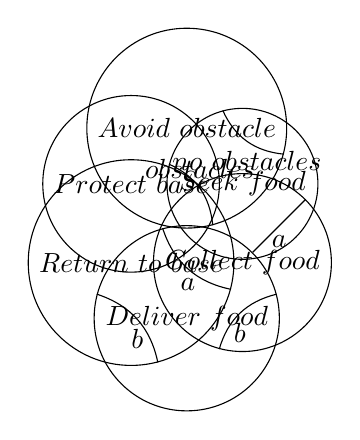
\begin{tikzpicture}
        \node[state] (1) {$Avoid\ obstacle$};
        \node[state, below left of=1] (2) {$Protect\ base$};
        \node[state, below right of=1] (3) {$Seek\ food$};
        \node[state, below of=3] (4) {$Collect\ food$};
        \node[state, below left of=4] (5) {$Deliver\ food$};
        \node[state, below of=2] (9) {$Return\ to\ base$};
        % \node[state, below  left of=1] (6) {$Flee\ enemy$};
        % \node[state, below  of=6] (7) {$Towards\ enemy$};
        % \node[state, below  of=7] (8) {$Attack\ enemy$};
        \draw
        (1) edge[below, bend left] node{$no\ obstacles$} (3)
        (3) edge[above, bend left] node{$obstacles$} (1)
        % (1) edge[below, bend right] node{$no\ obstacles$} (6)
        % (6) edge[above, bend right] node{$obstacles$} (1)
    
        (4) edge[below] node{$a$} (5)
        (5) edge[below, bend right] node{$b$} (4)
    
        (5) edge[below, bend right] node{$a$} (9)
        (9) edge[below, bend right] node{$b$} (5)
    
        ;
    \end{tikzpicture}
    \caption{Agent FSM}
    \label{fig:agent_FSM}
\end{figure}




\subsection{Behaviours} \label{subsection:behaviours}
Each agent has the ability to carry out a number of behaviours. 
The priority for carrying out the behaviours depend on the environment.
% When the environment is devoid of resources and threats, the agents wander in the perimeter of the home base.
If they encounter an obstacle, the aim is to avoid collision.
Failing to do so, they take damage until they get away from the obstacle.
When food is available, the agents start foraging, see Algorithm \ref{algorithm:seek}. 
A group of agents walks towards the food item, and collects it.
The agent that collected the mushroom, switches from foraging to delivering.
With a delivering task, the agent is entrusted to bring the mushroom back to the base.
When enough food is available at the base, the agents can return and stay at the base to replenish their health.
% Lastly, when there are threats in the environment, the agents need to be careful.
% If a snake comes close, the agent has to determine whether to flee \ref{algorithm:flee}, or to attack.
% The choice depends on availability of companions in the vicinity.
% Without other agents nearby, the agent flees, otherwise it attacks the enemy.
In all of the scenarios, the movements of the agents are affected by forces derived from their neighbors.
These forces include, alignment forces, cohesion forces and separation forces.


% https://en.wikibooks.org/wiki/LaTeX/Algorithms#Typesetting_using_the_algorithmic_package
% see buckland page 91 - 125
\subsubsection*{Seek}
The \textbf{seek} steering behaviour returns a force that directs an agent toward a target position.
% This behaviour is activated when the agent decides to attack the enemy.
% In our engine, this is determined by having the required number of neighbours in the vicinity.

\begin{algorithm}[H]
    \caption{Seek steering behavior}
    \begin{algorithmic}[1]
        \State desired\_velocity = target\_pos - agent\_pos
        \State desired\_velocity = normalize(desired\_velocity)
        \State \Return desired\_velocity
    \end{algorithmic}
    \label{algorithm:seek}
\end{algorithm}





\subsubsection*{Deliver}
The \textbf{deliver} steering behaviour is triggered when an agent collects a mushroom.
A force is returned that steers the agent towards the home base.

\begin{algorithm}[H]
    \caption{Food delivering steering behavior}
    \begin{algorithmic}[1]
        \State desired\_velocity = agent\_pos - target\_pos
        \State \Return desired\_velocity
    \end{algorithmic}
    \label{algorithm:deliver}
\end{algorithm}



\subsubsection*{Protect}
The \textbf{protect} steering behaviour is activated when the collective health of the swarm reaches a threshold.
Agents that are within the vicinity of the home base, stay inside the perimeter, 
while those that have wandered outside the perimeter return a force that steers them towards the base.

\begin{algorithm}[H]
    \caption{Base protection steering behavior}
    \begin{algorithmic}[1]
        \State desired\_velocity = agent\_pos - target\_pos
        \State \Return desired\_velocity
    \end{algorithmic}
    \label{algorithm:protect}
\end{algorithm}



% buckland p.99
\subsubsection*{Obstacle avoidance}
\textbf{Obstacle avoidance} aims to steer agents away from obstacles that are in their path.
The identification of two tiles are necessary for this behaviour; 
namely the tile on which the obstacle is placed and the tile on which the agent currently is located.
If the trajectory of the agent is towards the obstacle tile, and the distance is less than one tile;
then the obstacle avoidance behaviour is triggered.


\begin{algorithm}[H]
    \caption{Tile based obstacle avoidance steering behavior}
    \begin{algorithmic}[1]
        \State desired\_velocity = agent\_pos - target\_pos
        \State \Return desired\_velocity
    \end{algorithmic}
    \label{algorithm:avoid}
\end{algorithm}



\subsubsection*{Wander}
The \textbf{wander} steering behaviour returns a force that directs an agent towards a random location.
\begin{algorithm}[H]
    \caption{Wandering steering behavior}
    \begin{algorithmic}[1]
        \State desired\_velocity = agent\_pos - target\_pos
        \State \Return desired\_velocity
    \end{algorithmic}
    \label{algorithm:wander}
\end{algorithm}





% https://github.com/mdodsworth/pyglet-boids
\subsubsection*{Alignment}
\begin{algorithm}[H]
    \caption{Alignment collective steering behavior}
    \begin{algorithmic}[1]
        \State desired\_velocity = agent\_pos - target\_pos
        \State \Return desired\_velocity
    \end{algorithmic}
    \label{algorithm:alignment}
\end{algorithm}


In \textbf{alignment}, the velocity of an agent is manipulated to match that of its neighbours.

\begin{algorithm}[H]
    \caption{Alignment collective steering behavior}
    \begin{algorithmic}[1]
        \State desired\_velocity = agent\_pos - target\_pos
        \State \Return desired\_velocity
    \end{algorithmic}
    \label{algorithm:alignment}
\end{algorithm}



\subsubsection*{Cohesion}
\begin{algorithm}[H]
    \caption{Cohesion collective steering behavior}
    \begin{algorithmic}[1]
        \State desired\_velocity = agent\_pos - target\_pos
        \State \Return desired\_velocity
    \end{algorithmic}
    \label{algorithm:cohesion}
\end{algorithm}



The \textbf{cohesion} collective behaviour steers each agent to the geometric center of all nearby agents.

\begin{algorithm}[H]
    \caption{Cohesion collective steering behavior}
    \begin{algorithmic}[1]
        \State desired\_velocity = agent\_pos - target\_pos
        \State \Return desired\_velocity
    \end{algorithmic}
    \label{algorithm:cohesion}
\end{algorithm}



\subsubsection*{Separation}
\textbf{Separation} attemps to steer agents away from others, in order to prevent them crowding each other.
The algorithm iterates over all the perceived neighbours of the agent.
The vector to each neighbour is then normalized and divided by the distance to the neighbour.
This vector is then added to the steering force. 
\begin{algorithm}[H]
    \caption{Separation collective steering behavior}
    \begin{algorithmic}[1]
        \State desired\_velocity = agent\_pos - target\_pos
        \State steering\_force += normalized(distance\_to\_neighbour) / num\_neighbours
        \State \Return steering\_force
    \end{algorithmic}
    \label{algorithm:separation}
\end{algorithm}



\begin{algorithm}[H]
    \caption{Separation collective steering behavior}
    \begin{algorithmic}[1]
        \State desired\_velocity = agent\_pos - target\_pos
        \State steering\_force += normalized(distance\_to\_neighbour) / num\_neighbours
        \State \Return steering\_force
    \end{algorithmic}
    \label{algorithm:separation}
\end{algorithm}



\subsection{Swarm} \label{subsection:swarm}
The agents were grouped into a sprite group, called the swarm. 
A high level representation of the swarm is depicted in Figure \ref{fig:swarm}.
When an agent in the swarm reaches a health level of zero, it dies and is removed from the swarm.

\tikzset{
    ->, 
>=stealth, 
node distance=5cm,
every state/.style={thick, fill=gray!10},
initial text=$ $,}

\begin{figure}[H]
    \centering
    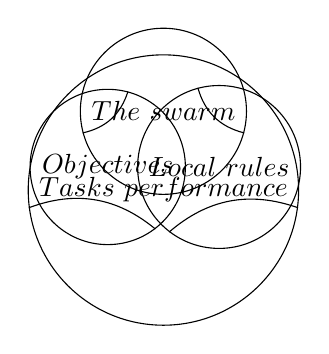
\begin{tikzpicture}
        \node[state] (1) {$The\ swarm$};
        \node[state, below right of=1] (2) {$Local \ rules$};
        \node[state, below  of=1] (3) {$Tasks\ performance$};
        \node[state, below left of=1] (4) {$Objectives$};
        \draw
        (1) edge[below, bend left] (2)
        (2) edge[below, bend left] (3)
        (3) edge[below, bend left] (4)
        (4) edge[below, bend left] (1)
    
        ;
    \end{tikzpicture}
    \caption{Swarm representation}
    \label{fig:swarm}
\end{figure}

% adapted from: Swarm Intelligence in Data Mining




\subsection{Food} \label{subsection:food}
The available food in the wilderness are mushrooms.
\textcolor{blue}{---
Consuming these mushrooms replenishes the energy and health of the agents. 
---}




\section{Results} \label{section:results}
% Results: simple past and present tense should be employed here, 
% but when you refer to figures and tables you use the present tense, 
% since they continue to exist in your paper ;); 
% you can mix active and passive voice.
\subsection*{Experiment 1: Degree of laziness}

The first experiment looks into the influence of offline allocation of tasks.
The task considered are foraging and staying.
The allocation is determined by a so-called laziness percentage.
This percentage decides how many agents should passively stay around the base, 
and the other agents are actively foraging for food.
For example, in a swarm of 20 agents, a percentage of 0.1 indicates that two agents stay behind while the remaining 18 forage.
Accordingly, 50\% indicates an equal allocation in numbers for the two tasks; i.e. ten agents each.
To determine the optimal ratio of staying to foraging in a swarm, 
the following experiment is proposed.

For each ratio ranging from 0 to 1, with 0.1 increments, the simulation is run.
The experiments are repeated 20 times for each strategy, after which an average is taken.
Two metrics are devised to measure the effectiveness of the strategies.

\begin{itemize}
    \item The average number of agents at the end of the simulation, for each laziness percentage.
    \item The average health of the remaining agents at the end of the simulation, for each laziness percentage.
\end{itemize}


% TODO: have a look at the results in kendall2004scripting.pdf
\textcolor{purple}{
    \blindtext
    \blindtext
}

\begin{figure}[H]
    \centering
    \includegraphics[width=0.75\textwidth]{graphics/results/lazyVSnum_agents.png}
    \caption{The fitness function of the population}
    \label{fig:lazy_vs_num_agents}
\end{figure}

\textcolor{purple}{
    \blindtext
    \blindtext
}

\begin{figure}[H]
    \centering
    \includegraphics[width=0.75\textwidth]{graphics/results/lazyVSavg_health.png}
    \caption{Survival rate of the population}
    \label{fig:lazy_vs_average_health}
\end{figure}

Figure \ref{fig:lazy_vs_num_agents} shows the average number of surviving agents for each strategy over the twenty runs.
Observed can be that a population comprised of solely lazy agents, those that do not forage at all,
lead to the worst survival rate.

In each of the twenty runs, no surivors were left.
This is logical, as the only way to survive is by foraging food.

By this logic however, one could assume that a population, consisting of foragers only, would fare the best.
This, as can be observed, has proven to be an incorrect assumption.

The resulting boxplot shows that the spread is large.
This can be addressed to the stochastic spawning of the mushrooms.
Some runs, may have seen enough mushrooms to allow many agents to survive, while other runs did not.

The very best strategy, according to this metric, would be 0.9, in which 18 members stay behind, while two look for food.
In all but one simulation, did every member survive.


Figure \ref{fig:lazy_vs_average_health} on the other hand shows the average health of the swarm at the end of the run for each strategy.
A measurement error can be observed in the strategy where 30 per cent of the swarm is lazy, as an average health of over 100 was reached at the end of the simulation.
This could be caused by an agent dying in the last moment of the simulation, and the calculation of the average health not taking it into account quick enough.

\textcolor{blue}{---
LIMITED CARRYING CAPACITY
---}

\textcolor{purple}{
    \blindtext
    \blindtext
}

\subsection*{Experiment 2: selfish vs unselfish}

In Figure \ref{fig:selfish_vs_num_agents} the number of surviving agents are shown for the selfish versus unselfish strategy.
A very clear result is obtained, in which the unselfish strategies far outperforms the selfish strategy.
However, the results obtained vary a lot in the unselfish group, which can directly be attributed to the limited availability of food.
The simulation also requires that sharing of the food only occurs if agents are close to the base.
In the case that every agent is actively searching for food to share, 
there will not always be a moment that there are many agents back at the base, as the mechanism is activated when a food item is collected.



\begin{figure}[H]
    \centering
    \includegraphics[width=0.75\textwidth]{graphics/results/selfishVSnum_agents.png}
    \caption{The surviving number of agents over 20 runs when either selfish or unselfish}
    \label{fig:selfish_vs_num_agents}
\end{figure}

\textcolor{purple}{
    \blindtext
    \blindtext
}

In Figure \ref{fig:selfish_vs_average_health} the average health achieved by the surviving agents is plotted.
Observed can be that there is more variety in the selfish population.
This can be directly attributed to the lower survival rate.


\begin{figure}[H]
    \centering
    \includegraphics[width=0.75\textwidth]{graphics/results/selfishVSavg_health.png}
    \caption{The average health of the surviving number of agents over 20 runs when either selfish or unselfish}
    \label{fig:selfish_vs_average_health}
\end{figure}

\textcolor{purple}{
    \blindtext
    \blindtext
}
\section{Discussion} \label{section:discussion}
% Discussion: use the simple past for your own findings 
% and the perfect tense for cited information; 
% the present tense is also acceptable, 
% if you prefer that one (in such statements as ‘We can conclude that …’.
In this work, we have presented a novel engine for the development of swarm intelligence.
Self-organizating behaviours in the context of task allocation has been demonstrated.

\textcolor{purple}{
    \blindtext
    \blindtext
}
\textcolor{purple}{
    \blindtext
    \blindtext
}

Refer to chapter \ref{subsection:goals} that defines the goals of our thesis. 
We have achieved all of our goals in this thesis. 
Therefore, we can identify the following contributions to research

\begin{enumerate}
    \item In chapter \ref{section:background} we motivated work on swarm intelligence in video games by highlighting relevant work in the field of Game AI.
    In particular we looked into real time strategy games.
    \item In chapter \ref{section:methodology} we documented the methods to develop a multi-agent survival game engine, in which swarm intelligence can be implemented.
    \item in chapter \ref{subsection:agent} we showed how Finite State Machines could be used to implement self-organized behaviour in a swarm of individually controlled agents, with a focus on task allocation.
    % \item In chapter \ref{subsection:evaluation_metric} we also showed how evolutionary computing can be applied to swarm intelligence.
\end{enumerate}

\subsection*{Motivating work on swarm intelligence}
\textcolor{purple}{
    \blindtext
    \blindtext
}

\subsection*{The game engine}
\textcolor{purple}{
    \blindtext
    \blindtext
}

\subsection*{Self-organized behaviour}
\textcolor{purple}{
    \blindtext
    \blindtext
}

% \subsection*{Evolving the swarm}
\textcolor{purple}{
    \blindtext
    \blindtext
}

\subsection{Limitations} \label{subsection:limitations}
% The hardware on which the simulation was developed was not optimal.

\subsection*{Motivating work on swarm intelligence}
\textcolor{purple}{
    \blindtext
    \blindtext
}

\subsection*{The game engine}
The main limitation presented by the game engine, is the difficulty in scaling.
Pygame is not intended to be used to simulate a large number of agents, and as such it showed, 
as with increasing numbers, the game became much slower and less reactive.
Ultimately, this is acceptable, as the engine developed is intended for academic purposes solely, 
however for more elaborate research, either hardware with stronger capabilities is needed, 
or the game needs to be ported to engines more capable of handling multi-agent environments.

% One could look into engines such as unity, 
\textcolor{purple}{
    \blindtext
    \blindtext
}

\subsection*{Self-organized behaviour}
\textcolor{purple}{
    \blindtext
    \blindtext
}



\subsection{Future work} \label{subsection:future_work}
Future work concerning the proposed framework, should focus on adding more complexity to the simulation.
This could be achieved by adding more challenging elements to the environment, such as bodies of water, bridges and fire.
Furthermore, the use of procedural content creation could prove useful, especially in training as the current implementation has a predictable environment due to the perlin noise.

\textcolor{purple}{
    \blindtext
    \blindtext
}
\section{Conclusion} \label{section:conclusion}
% Conclusions and Further work: 
% use present perfect to make clear that your statements 
% still hold at the time of reading; 
% for further work the future tense (or the present) is acceptable.

In this work, we have presented a novel engine for the development of swarm intelligence.
Self-organizating behaviours in the context of task allocation has been demonstrated.

\textcolor{purple}{
    \blindtext
    \blindtext
}

\newpage
\begin{appendices}
    \input{sections/appendices/A.tex}
\input{sections/appendices/B.tex}
\end{appendices}
\newpage

\bibliographystyle{unsrt}
\bibliography{./references}

\end{document}